\documentclass[a4paper,11pt]{article}

\usepackage[utf8]{inputenc}
\usepackage[T1]{fontenc}
% Utilisons palatino pour plaire à certains afficheurs de PDF
\usepackage{pxfonts} 
\usepackage{fancyhdr}
\usepackage{moreverb}
\usepackage{tocbibind}
\usepackage{geometry}
\usepackage{graphicx}
%\usepackage{rcs}
\usepackage{hyperref}
\usepackage[french]{babel}
\usepackage{listings}
\usepackage{url}
\usepackage{ulem}
\lstset{
    language=bash, %% Bon défaut dans notre cas
    inputencoding=utf8,
    literate=%
    {é}{{\'e}}1%
    {è}{{\`e}}1%
}
\usepackage{supertabular}

\usepackage{datetime2}
\usepackage[local]{gitinfo2}

% format de la date pour Git
\DTMnewdatestyle{mydate}{%
  \renewcommand*{\DTMdisplaydate}[4]{##3 \DTMfrenchMonthname{\DTMtwodigits{##2}} ##1}%
  \renewcommand{\DTMDisplaydate}{\DTMdisplaydate}%
}
\DTMsetdatestyle{mydate}

% definition du format de l'entete et du pied de page
\pagestyle{fancyplain}
\lhead{}
\rhead{\leftmark}
\rfoot{
  \begin{scriptsize}
  \textsl{version du \DTMusedate{gitdate}}
  \end{scriptsize}
}

%%% warning encadré
%%% utilisation : \begin{warning} blablabla \end{warning}
\usepackage{pifont,mdframed}
\newenvironment{warning}
  %%{\par\begin{mdframed}[linewidth=2pt,linecolor=red]%
  {\par\begin{mdframed}[linewidth=2pt]%
    \begin{list}{}{\leftmargin=1cm
                   \labelwidth=\leftmargin}\item[\Large\ding{43}]}
  {\end{list}\end{mdframed}\par}

%%% pour l'usage des programmes qui ne tiennent pas sur une ligne
%%% utilisation :
%%%%%% \minibox[frame]{
%%%%%%  \texttt{gengraphvect\.py [-h] -a ACQID [-o FORMAT] [-n NIVEAU]} \\
%%%%%%  \rightline{ \texttt{[-f FICHIER] [-s SENS] [-v] [VECTEUR ...]} }
%%%%%% }
\usepackage{minibox}


\hypersetup{
       colorlinks=true,%  Liens en couleur 
       linkcolor=blue,%   Liens bleus
       urlcolor=blue,%   Liens bleus
       %%hyperindex=true,%  Ajoute des liens dans les index.
       pdftitle={Documentation AIDA Volume 3 : Guide du développeur et de l'administrateur},
       pdfauthor={CNRM/GMEI/TRAMM - SAFIRE},
       pdfkeywords={Guide du développeur et de l'administrateur}
}

% Let's have some nice headings
\addtolength{\headheight}{2.3pt}
\title{Documentation AIDA \\Volume 3 : Guide du développeur et de l'administrateur}
\author{CNRM/GMEI/TRAMM \and SAFIRE}
\date{Version du \DTMusedate{gitdate}}

\begin{document}
\maketitle
\newpage

\tableofcontents
\newpage

\section*{Présentation}
	Le guide du développeur regroupe les informations nécessaires à :
\begin{itemize}
  \item installer AIDA sur une machine,
  \item écrire un programme spécifique (application personnelle),
  \item modifier un des programmes d'usage général (adc, aidaplot, vec2asc, ...).
\end{itemize}
Il décrit les méthodes de travail choisies, et les outils disponibles.
Il est divisé en plusieurs chapitres :
\begin{itemize}
  \item \nameref{part:install},    page \pageref{part:install}
  \item \nameref{part:dev_C},      page \pageref{part:dev_C}
  %% \item Développements avec R  page \pageref{part:dev_R}
  \item \nameref{part:dev_Python}, page \pageref{part:dev_Python}
  \item \nameref{part:dev_sh},     page \pageref{part:dev_sh}
\end{itemize}


% Partie 1 : Diffusion et installation
\part{Distribution et installation}
\label{part:install}

%% On compte sur la commande path du package url
\newcommand{\pathfmt}[1]{\path{#1}}
\newcommand{\clavier}[1]{\texttt{#1}}

  Les bibliothèques de fonctions qui sont au c\oe{}ur du système AIDA
(manipulation de fichiers, traitements) sont écrites en langage C et en
langage Python.

\section{Pré-requis}
  Pour installer et utiliser les différents programmes qui constituent
AIDA sur une machine, celle-ci doit offrir un certain nombre de
services. Ce sont :

\begin{description}
  \item[un système de développement \texttt{C-ANSI}] : un compilateur, un
    éditeur de liens, les programmes \texttt{make} et \texttt{makedepend}.
    AIDA est développé avec les versions standard disponibles sur la
    distribution GNU/Linux \textbf{Ubuntu} (architecture x86\_64),
    avec gcc et clang.

  \item[python] : les programmes python dans AIDA sont compatibles avec la
    version installée en standard sur Ubuntu. La présence des packages
    nécessaires est testée par l'installateur de AIDA.

  \item[\LaTeX] : cette documentation, et les documentations des fonctions de
    traitement («opérateurs») sont écrites en \LaTeX.

  \item[la bibliothèque udunits2] : c'est une bibliothèque de manipulation
    d'unités développée par le groupe \textit{UNIDATA}. Dans AIDA,
    elle sert, par exemple, à vérifier que l'unité d'un vecteur correspond
    bien à ce que le programme de traitement attend.

  \item[la bibliothèque lapack (et blas)] : Lapack (\textbf{L}inear
    \textbf{A}lgebra \textbf{PACK}age), est une bibliothèque de routines
    Fortran 77 utilisée pour résoudre des problèmes d'algèbre
    linéaire : résolution de systèmes linéaires, problèmes de moindres carrés,
    problèmes aux valeurs propres, factorisations de matrice, ...

  \item[la bibliothèque Z] : la bibliothèque zlib permet de compresser ou de
    décompresser des données en mémoire ou de lire et écrire des fichiers au
    format gzip.

  \item[cextract] : ce programme génère automatiquement les prototypes de
    fonctions écrites en langage C. Ce programme n'est donc nécessaire
    \emph{que lors de modifications des sources}. Il n'est pas nécessaires
    pour une utilisation courante. L'auteur est Adam Bryant (adb@bu.edu). AIDA
    utilise la version 1.7, qui date de 1992.
    Ce programme qui a été diffusé sur le newsgroup
    \texttt{comp}\texttt{.sources.reviewed}, et que l'on pouvait trouver à
    \url{http://www.cs.bu.edu/ftp/pub/adb/}, ou inclus dans divers packages
    logiciels, par exemple les sources de Thot
    (\url{http://www.inrialpes.fr/opera/Thot/index.html}) a été enregistré
    dans \$AIDA\_HOME/extern/src/.  Il est accompagné de
    \texttt{cextdoc}, générateur automatique de documentation, qui n'est plus
    utilisé dans AIDA.
    Si les difficultés d'utilisation deviennent trop grandes,
    une alternative serait Makeheaders (\url{http://www.hwaci.com/sw/mkhdr/})

  \item[doxygen] : doxygen est un logiciel permettant de générer de la
    documentation technique à partir du code source d'un programme.
    Il extrait les déclarations et certains commentaire du code source,
    et crée un manuel de référence (format HTML, ou pdf via LaTeX),
    pour permettre au programmeur de localiser rapidement une fonction
    ou une structure quelconque. C'est un logiciel libre.

\end{description}

D'autres outils peuvent être nécessaires pour des applications qui ne sont pas
utilisées partout :

\begin{description}
  \item[Labview] : LabVIEW est un logiciel de développement d'applications
    par programmation graphique. Il est développé et vendu par la
    société américaine National Instruments (\url{http://www.ni.com/labview/f/}).
    Il est principalement orienté vers les tests, la mesure et
    l'automatisation, mais il permet aussi de développer des applications
    d'analyse de données.

  \item[la bibliothèque netcdf] : elle sert à lire et écrire des fichiers au
    format NetCDF, et ne sera utile que si vous avez à manipuler des fichiers
    à ce format.

  \item[graphviz] : logiciel de visualisation de graphes
    \url{http://www.graphviz.org/}.

\end{description}


\section{Modes de distributions et installation}

La méthode de distribution de AIDA est basée sur un fichier \texttt{tar}.
%%%Se repporter à la documentation \texttt{\textbf{installateur\_aida.pdf}}.
Se repporter à la documentation \url{installateur\_aida.pdf}.



% Partie 2 : Infos générales sur le Développement
\part{Choix généraux d'organisation des développements}
\label{part:dev_gene}

Cette partie traite du cadre général des développement dans AIDA, c'est à dire
l'écriture (ou la modification) de programme ou fonction d'usage général, de
documentation, mais pas l'utilisation d'AIDA pour effectuer tel ou tel
traitement.

Les sources sont stockés dans un système de gestion
de source (\texttt{git}).

%% problème avec dev.bib  : remplacement de \cite{Miller1997} par l'url seule
Le processus de compilation/installation est basé sur l'utilisation récursive
de make\footnote{\label{make}Cette technique est controversée, notamment par
Peter Miller, qui explique pourquoi les make récursifs ne permettent pas de
voir l'arbre complet des dépendances, et obligent soit à en négliger certaines,
soit à faire du travail en double
(\url{http://aegis.sourceforge.net/auug97.pdf}).  AIDA n'est pas un gros projet
(au sens de P. Miller) et on parvient à faire une compilation ordonnée
(bibliothèques avant programmes) qui évite les dépendances complexes.}
sur toute l'arborescence AIDA.


\section{Utilisation des makefile}
\label{sec:make}

\subsection{Cibles usuelles}
Chaque makefile devra définir au moins trois cibles  :

\begin{description}
  \item[clean] : supprime tous les fichiers générés au cours du processus de
    construction.
  \item[depend] : calcule les dépendances qui peuvent être construites
    automatiquement.
  \item[install] : construit le résultat attendu (bibliothèque, programme,
    document, ...) dans le répertoire actuel puis copie le résultat vers un
    répertoire
    (\texttt{\$AIDA\_HOME/lib, \$AIDA\_HOME/bin, \$AIDA\_HOME/doc, ...}).
\end{description}
\bigbreak

Il est souhaitable que le makefile définisse la cible \texttt{\textbf{all}} :
\begin{description}
  \item[all] : construit le résultat attendu (bibliothèque, programme,
    document, ...) dans le répertoire actuel (le plus souvent, "all" est la
    cible par défaut).
\end{description}
\bigbreak

Une cinquième cible, \texttt{\textbf{check}}, qui exécute des tests, est pour
l'instant recommandée mais pas encore systématique.


\subsection{Configuration et portabilité}
Pour éviter d'effectuer au sein de chaque makefile une reconnaissance de la
machine hôte, et une adaptation à l'environnement local (versions et options
des compilateurs et autres utilitaires), ces réglages sont regroupés dans un
fichier unique \path{$AIDA_HOME/config/local_cfg.mk}, et tous les makefiles
incluent ce fichier de configuration grâce à la ligne :
\smallbreak
\begin{boxedverbatim}
-include $(AIDA_HOME)/config/local_cfg.mk 
\end{boxedverbatim}
\medbreak

Le fichier \path{$AIDA_HOME/config/local_cfg.mk} contient toutes les
définitions de macros pouvant être différentes selon l'environnement. C'est un
lien sur :\\
\path{AIDA_HOME/local/make/Linux_$DISTRIB_$DISTRIB_RELEASE_$ARCH.auto.mk}. \\

Le fichier
\path{AIDA_HOME/local/make/Linux_$DISTRIB_$DISTRIB_RELEASE_$ARCH.auto.mk} et
le lien \path{$AIDA_HOME/config/local_cfg.mk} sont générés automatiquement par
l'installateur (voir : \path{$AIDA_HOME/scr/script/set_make_config.sh})

\subsection{Quelques points techniques spécifiques}
\begin{itemize}
\item Pour compatibilité avec
un système de gestion de sources,
les dépendances générées automatiquement par
makedepend ne sont pas écrites en fin de makefile,
mais dans un fichier séparé.
%TODO : explication de la technique
\item .SECONDEXPANSION pour gmake version $\geq$ 3.81
\end{itemize}



% Partie 3 : Développements en C
\part{Développements en langage C}
\label{part:dev_C}

\textbf{\textit{note : le codage en langage C est abandonné au profit du codage
en langage Python.}}

\section{Règles de codages}
   AIDA est pour l'instant un petit projet, qui ne concerne pas un
grand nombre de programmeurs. Nous n'avons donc pas mis en place
de règles de codages strictes. Ce n'est pas une raison pour écrire
du code incompréhensible, non-portable, ... Il est donc fortement
recommandé de connaître une des règles de codages existantes
(par exemple, le «GNU Coding standard» 
\footnote{\url{http://www.gnu.org/prep/standards_toc.html}})
, et de la suivre, sinon \`a la lettre, du 
moins dans les grands principes.

  Pour uniformiser la présentation et faciliter la (re)lecture
des sources, l'usage s'est répandu (et même systématisé à TRAMM)
d'automatiser la mise en forme des sources avec l'utilitaire \texttt{indent}.

  Les commentaires seront rédigés de manière à faciliter la
création d'une documentation technique par des outils automatiques.
Actuellement, la recommandation est d'utiliser l'outil
Doxygen\footnote{\url{https://www.doxygen.nl/}},
avec style de commentaires se
rapprochant de javadoc\footnote{\url{http://fr.wikipedia.org/wiki/Javadoc}}.
Historiquement, la documentation automatique des premiers programmes (la 
bibliothèque \texttt{rapt}, par exemple) était faite avec l'outil
\texttt{cextract/cextdoc}.
Certains commentaires «ancien style» persistent donc encore
dans les sources.


\section{La bibliothèque \texttt{rapt}}
\label{sec:rapt}
   Un certain nombre de fonctions utilisées fréquemment dans
l'environnement AIDA (lecture/écriture d'un vecteur, codage
ou décodage d'un "AcqId", ...) ont été rassemblées dans une 
bibliothèque, baptisée \textit{rapt}\footnote{Historiquement,
cela signifiait \textit{Research Aircraft Processing Tools}}.
Voici une présentation générale des différents groupes de fonctions
(une présentation détaillée de chaque fonction, avec le type
de chaque argument, et un court texte descriptif se trouve
dans le fichier \texttt{rapt.doc.ps} du répertoire 
\path{$AIDA_HOME/src/lib/rapt}).

\subsection{Fonctionnement général et traitement des erreurs}
  Cette bibliothèque fonctionne selon un système semblable à 
celui de la bibliothèque standard pour les appels systèmes en C. En cas
d'erreur, la fonction retourne une valeur invalide (indice
négatif, pointeur NULL, ...) et une variable globale 
précise le type d'erreur.

  Dans cette bibliothèque, la variable globale s'appelle \texttt{errapt},
et les fonctions \texttt{strerrapt()} et \texttt{perrapt()} permettent
d'obtenir, respectivement, une chaîne de caractère ou 
l'écriture d'un message décrivant l'erreur.

\subsection{Manipulation des types connus par AIDA}
\begin{description}
  \item[AidaTypCode()] : sert à reconnaître un nom de format : reçoit une
    chaîne de caractère, et renvoie le code correspondant (membre de l'enum
    \texttt{AIDA\_TYPE\_CODE)}.
  \item[AidaTypNom()] : fournit les noms (chaîne de caract. ) des types
    standard connus de AIDA (symétrique de AidaTypCode()).
  \item[AidaTypSize()] : fournit la taille (en octet) des types standard
    connus de AIDA.
\end{description}

\subsection{Manipulation des "AcqId" (noms uniques de chaque série de mesure)}
\begin{description}
  \item[Full2Id() :] construit un "Identificateur d'acquisition" (AcqId)
à partir des informations unitaires (nom de plate-forme, année, numéro
d'acquisition dans l'année).
  \item[Id2DataPath() :] construit le chemin du répertoire contenant les
données d'une acquisition.
  \item[Id2Full() :] fournit les informations unitaires (nom de plate-forme,
 année, numéro d'acquisition dans l'année) à partir de l'identificateur
d'acquisition" (AcqId).
\end{description}

\subsection{Utilisation des variables d'environnement}
         Le principe général est qu'une seule variable 
d'environnement (\texttt{AIDA\_HOME}) est nécessaire, mais
que d'autres variables (\texttt{AIDA\_LIB},  \texttt{AIDA\_DATA}, ...)
permettent de travailler sur des répertoires particuliers. La fonction
\texttt{AidaGetEnv()} gère automatiquement ce système
de valeurs particulières qui peuvent remplacer une valeur
par défaut.

\subsection{Travail sur les en-têtes}
            fonctions GetHdrValxxx, SetHdrValxxx

\subsection{Travail sur les données}
            fonctions AccessVectData, AllocVectData, FreeVectData

\section{Écriture d'un opérateur}
\label{sec:ecr_oper}

\textbf{\textit{note : le développement d'opérateurs en langage C est
abandonné au profit du développement d'opérateurs en langage Python (voir :
\nameref{sec:adc_oper}, page \pageref{sec:adc_oper}) \\
Cependant les opérateurs développés en langage C sont exécutables par
l'interpréteur de commande \texttt{adc} (voir \url{user.pdf})}}
\bigbreak

   Un opérateur, dans l'environnement AIDA, c'est une fonction
compilée, incluse dans une bibliothèque à chargement dynamique, qui travaille
sur une série temporelle de données (la notion de vecteur), avec les
fonctions d'interfaçage nécessaire pour être utilisée par l'interpréteur
de commandes adc 
(ou tout autre programme utilisant la même interface d'appel comme l'ancien
interpréteur fvb).

Concrètement, un opérateur est l'association de quatre choses :
\begin{itemize}
  \item une fonction, qui fait effectivement les calculs. Généralement en
    C ou en Fortran. Cette fonction peut faire appel à d'autres fonctions, ou
    à des bibliothèques.
  \item une fonction d'interface, qui permet à toutes les fonctions
    de pouvoir être appelées avec une même syntaxe d'appel (liste et types
    d'arguments).
  \item une fonction de documentation, qui remplit une structure décrivant
    l'opérateur et ses arguments.
  \item la documentation (format \LaTeX ).
\end{itemize}

\subsection{Le code-source d'un opérateur}
La convention de nommage est la suivante : pour un opérateur
dont le nom est <nom\_oper>, les sources sont dans un
fichier <nom\_oper>.c, qui contient la fonction d'interface
OP\_<nom\_oper> et la fonction de documentation ID\_<nom\_oper>.
La plupart du temps, la fonction qui fait le calcul est dans le
même fichier et s'appelle  <nom\_oper>, mais il peut y avoir
des exceptions lorsqu'une seule fonction peut être appelée
par deux opérateurs distincts\footnote{Par exemple, l'opérateur
Plus\_flt fait appel à la fonction de calcul Plus qui est
définie dans le source de l'opérateur Plus}
\footnote{Une autre exception est le fichier Tair.c, qui 
contient les fonction Tair, OP\_Tair et ID\_Tair, 
ainsi que OP\_Tair\_avion et ID\_Tair\_avion, qui définissent
l'opérateur Tair\_avion, mais ne font rien d'autre qu'un appel
à Tair avec une liste d'arguments spécifique}.


\subsubsection{Spécifications des propriété des vecteurs produits}
    La fonction ID\_<nom\_oper> retourne un tableau de structures,
dont chaque élément décrit un argument, et en spécifie les
attributs.

\begin{tabular}{l|l|l}
 nom          & type   & description  \\
\hline
nom	& Chaîne & \\
\hline
nom anglais	& Chaîne & \\
\hline
array\_dim	& float\_64 & \\
\hline
sample	& float\_64 & \\
\hline
NbVal	& float\_64 & \\
\hline
unit	& Chaîne & \\
\hline
ref\_time	& float\_64 & \\
\hline
misval	& float\_64 & \\
\hline
famille	& Chaîne & \\
\hline
\end{tabular}

\subsection{Écriture de la documentation d'un opérateur}

  La documentation d'un opérateur est écrite en \LaTeX, et répartie en
trois fichiers : les sections spécifiques à la description des arguments
et à la formule (ou l'algorithme) employée sont écrites dans des fichiers
séparés,
qui seront inclus dans le document général, mais qui peuvent aussi être
réutilisés et inclus dans
d'autres documents (rapports de traitement, ...)

   Comme tous les sources LaTeX, ces fichiers sont de simples fichiers
textes, modifiables avec des éditeurs généralistes (vi, emacs) ou
spécialisés (TexMaker, ...). Les
accents des textes contenus dans ces fichiers doivent être codée en
ISO-8859-15
\footnote{ISO-8859-15 est aussi baptisé
"latin9", et quasi-équivalent, pour notre usage, au
« code page » cp1252 de Windows.}.
Si vous êtes dans un environnement de travail où il est
impossible de configurer
un éditeur pour travailler en ISO-8859-15, il est toujours possible de
saisir les accents
« à l'ancienne », c'est à dire \clavier{\textbackslash'e} pour é, 
\clavier{\textbackslash`a} pour à, ...

Ces fichiers résidents dans le répertoire \pathfmt{AIDA_HOME/src/doc/oper}. Par
convention, pour un opérateur baptisé
<oper>, le fichier principal sera \pathfmt{<oper>.tex}, le fichier de
description des arguments sera \pathfmt{arguments/<oper>.args.tex},
et le fichier de description des formules sera
\pathfmt{formules/<oper>.frm.tex}. 
Enfin, pour pouvoir produire
des documentations de traitement en anglais, 
il est nécessaire qu'une version anglaise de la formule 
soit rédigée dans le fichier :
\pathfmt{formules/<oper>.frm.en.tex}.

 Il n'est jamais nécessaire de créer ces fichiers à partir de rien. Si
l'opérateur que l'on vient de créer ressemble à un opérateur existant,
il suffira de copier et modifier les fichiers de
cet opérateur.
Sinon, il existe un programme qui sait créer un squelette de
documentation : il se trouve
dans le répertoire \path{$AIDA_HOME/src/lib/oper/} et il s'appelle
\texttt{oper2doc}.

Dans le premier cas, l'effort de modification de la description peut
être minime, mais il
faut être attentif aux changements techniques (nombre, ordre et unité
des arguments).
Dans le second cas, la liste des arguments (et leurs propriétés : type,
catégorie, unité) créée
automatiquement sera parfaitement exacte, mais sans aucune intelligence
: les noms
seront Arg1, Arg2, Argn, et la formule sera vide.

La plupart du temps, il n'est pas nécessaire d'être expert en
\LaTeX{} pour écrire la documentation. Si besoin est, une
rapide introduction à l'écriture de mathématiques en
\LaTeX{}  se trouve sur le site des tuteurs de l'ENS :
\url{http://www.tuteurs.ens.fr/logiciels/latex/maths.html}.
Il faut être attentif à quelques points :\begin{itemize}
\item Les noms des variables utilisés dans la formule
doivent correspondre aux noms donnés dans la liste des
arguments.
\item Il ne faut pas utiliser la commande 
\clavier{\textbackslash\textbackslash} pour forcer 
un changement de ligne de texte, car celle-ci devient une fin 
de ligne de tableau si le fichier est inclus dans une
cellule d'un tableau. Les méthodes recommandées
sont d'utiliser le mode math hors-texte ( \verb+\[ ... \]+ ),
ou le changement de paragraphe
canonique (ligne vide).
Au pire, utiliser \clavier{\textbackslash{}newline}
\end{itemize}

\noindent Il faut ensuite :\begin{itemize}
 \item Modifier le fichier \pathfmt{CATALOG_OPER.tex} pour ajouter 
une ligne \newline
\clavier{\textbackslash input\{<nom\_oper>\}\textbackslash newpage}
dans le chapitre adapté.
 \item Produire la nouvelle
version de \pathfmt{CATALOG_OPER.pdf} par la commande \newline
\clavier{make  CATALOG\_OPER.pdf}
 \item Itérer les actions d'édition/compilation/relecture jusqu'à
  satisfaction
 \item Éventuellement, tester si la documentation qui vient d'être
écrite est bien utilisable pour générer la documentation automatique
d'un traitement. Pour cela, il faut qu'un vecteur ait été calculé
avec l'opérateur, créer un petit fichier texte contenant 
le nom de ce vecteur, puis exécuter :\newline
\clavier{mk\_doctrt <AcqId> <nom\_du\_fichier\_texte> /tmp/TEST\_DOC}
 \item Enregistrer les fichiers dans le système de gestion 
de code ("\clavier{commit}").
\end{itemize}


% Partie 4 : Développements avec R
%% \part{D\'eveloppements avec R}
\label{part:dev_R}

\section{Bibliothèques de fonctions}
  Les fonctions les plus fréquement utilisées sont regroupées dans des
bibliothèques. 
~


% Partie 5 : Développements avec Python
\part{Développements avec Python}
\label{part:dev_Python}

\section{Généralités}
Les développements sont en \textbf{\texttt{Python3}} et rassemblés dans le
répertoire : \\
\-\hspace{1cm} \path{$AIDA_HOME/src/python3}.
\smallbreak

  Le code est indenté par 4 espaces (et non pas le caractère TAB). Il peut être
nécessaire de régler votre éditeur préféré afin qu'il insère 4 espaces lorsque
la touche TAB est tapée.
\smallbreak

  Les codes python doivent débuter par le sheebang :
\begin{boxedverbatim}
#!/usr/bin/env python3
\end{boxedverbatim}
\smallbreak

La documentation, générée par \texttt{sphinx}, est sous : \\
\-\hspace{1cm} \path{$AIDA_HOME/doc/sphinx/html/index.html}.

\section{Règles de codages}
   Il est vivement conseillé de suivre les conventions de codage usuelles du
monde Python, formalisées dans le PEP-8
\footnote{\url{http://www.python.org/dev/peps/pep-0008/}},
et vérifiables par pylint\footnote{\url{http://www.pylint.org/}}.
\smallbreak

  Le code écrit pour AIDA doit être (autant que faire se peut) indépendant de
la plateforme. En particulier, la construction des noms de répertoire et de
fichier doit être faite en utilisant la méthode \textbf{\texttt{os.path.join}}.
En aucun cas le séparateur \texttt{/} ne doit être explicitement utilisé.
\smallbreak

  En aucun cas la variable d'environnement \texttt{PYTHONPATH} ne doit être
utilisée, que ce soit de façon implicite ou explicite
(voir : \nameref{sec:import_AIDA}, page \pageref{sec:import_AIDA}). \\
\smallbreak

Il est vivement recommandé de coder un \textit{main} dans les modules afin de
permettre de \textbf{tester le code} :
\begin{boxedverbatim}
if __name__ == '__main__':
\end{boxedverbatim}


\section{Les modules de AIDA}
  Les modules de \textbf{AIDA} rassemblent les outils (fonctions, classes)
utiles pour travailler dans un environnement AIDA. Ils sont regroupés sous le
répertoire : \\
\-\hspace{1cm} \path{$AIDA_HOME/src/python3/AIDA_lib}

\medbreak
\textbf{Afin de faciliter la maintenance du code AIDA, ces modules
doivent être utilisés par les programmes développés dans le cadre du projet}.

\subsection{Utilisation des modules de AIDA}
\label{sec:import_AIDA}
  Tout programme souhaitant utiliser les modules de AIDA doit modifier
\textbf{explicitement} la variable de recherche des modules avant d'importer
les modules désirés.
Le système d'installation de AIDA copie les modules dans le répertoire : \\
\-\hspace{1cm} \path{$AIDA_HOME/lib/python<num_version>}. \\
Ce sont ces copies qui doivent être importées par l'utilisation du code
suivant :

\medbreak
\begin{boxedverbatim}
import os
import sys

PYTHON_X_Y = 'python%d.%d' % (sys.version_info[0], sys.version_info[1])
sys.path.append(os.path.join(os.getenv('AIDA_HOME'), 'lib', PYTHON_X_Y))

import ...

\end{boxedverbatim}

\subsection{Documentation des modules de AIDA}
  Afin que la documentation d'un module de AIDA apparaise dans la documentation
générale, il convient de la faire générer par \texttt{sphinx}. \\
Pour cela, il suffit d'ajouter une section au fichier : \\
\-\hspace{1cm} \path{$AIDA_HOME/src/doc/sphinx/source/modules_python.rst}


\subsection{Le module \emph{AIDA.py}}
  Les éléments principaux sont :
  \begin{itemize}
    \item[•] La classe Vector
    \item[•] La classe Inf
    \item[•] des fonctions liées aux conventions AIDA
      \subitem - \texttt{Y2\_to\_Y4},
      \subitem - \texttt{AIDA\_freq\_fmt},
      \subitem - \texttt{AIDA\_abrev\_to\_family},
      \subitem - \texttt{AIDA\_abrev\_to\_plt},
      \subitem - \texttt{AIDA\_long\_to\_abrev}
    \item[•] des fonctions d'utilisation des indicateurs d'acquisition
      \subitem - \texttt{ID\_to\_full},
      \subitem - \texttt{ID\_to\_relpath},
      \subitem - \texttt{ID\_to\_datapath},
      \subitem - \texttt{ID\_to\_infpath},
  \end{itemize}

  Voir la documentation complète :  \\
\-\hspace{1cm} \path{$AIDA_HOME/doc/sphinx/html/index.html}.


\section{Écriture d’un opérateur}
\label{sec:adc_oper}

  Pour des raisons historiques, un opérateur, dans l'environnement AIDA, peut
être de deux natures :
  \begin{itemize}
    \item[•] codé en Python
    \item[•] codé en C
             (voir \nameref{sec:ecr_oper}, page \pageref{sec:ecr_oper}).
  \end{itemize}

\medbreak
  Un opérateur a pour vocation d'être appelé par l'interpréteur de commande de
AIDA : \texttt{adc}. Cependant, il pourrait être appelé par tout autre
programme utilisant la même interface d'appel. Dans la suite de cette
documentation le seul vocable \texttt{adc} sera utilisé.

\medbreak
  Un opérateur Python est constitué de 4 parties :
  \begin{itemize}
    \item[•] une fonction de caclul.
    \item[•] une fonction d'interface entre la fonction de calcul et
             \texttt{adc}.
    \item[•] une description de la fonction d'interface.
    \item[•] une documentation.
  \end{itemize}

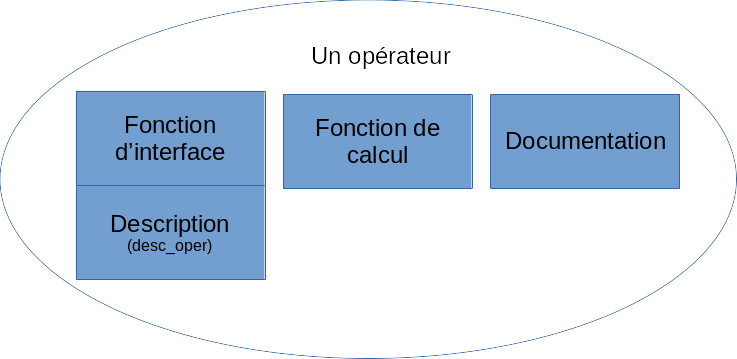
\includegraphics[scale=0.5]{images/schema_oper.png}

\subsection{une fonction de caclul}
  C'est une fonction Python qui effectue un traitement sur une série
  temporelle de données : les données d'un vecteur. \\

  Généralement elle reçoit les données des séries temporelles et retourne ses
  résultats sous forme de tableaux \texttt{numpy}. \\

  Les fonctions de calcul sont regroupées sous : \\
  \-\hspace{1cm} \path{$AIDA_HOME/src/python3/packages/calcul}.  \\

  (voir : \nameref{sec:ex_fct_calcul}, page \pageref{sec:ex_fct_calcul}). \\

  Si le code du module contient un \textit{main}, son code doit permettre de
  \textbf{tester la fonction de calcul}.


\subsection{une fonction d'interface}
  C'est une fonction Python qui fait l'interface entre la fonction de calcul
  et \texttt{adc}. \\

  Ses paramètres d'entrée sont des objets AIDA \textbf{\texttt{VectorMask}},
  des \textbf{\texttt{coefficients}}. \\

  Cette fonction Python peut déclarer des paramètres optionnels selon les
  principes de la programmation Python. \\

  Le code de la fonction d'interface est divisé en 4 phases :
  \begin{itemize}
    \item[•] préparation des arguments pour appeller la fonction de calcul.
    \item[•] appel de la fonction de calcul.
    \item[•] préparation du/des header(s) du/des vecteur(s) de retour.
    \item[•] préparation du diagnostique d'exécution.
  \end{itemize}
\medbreak

  Elle retourne ses résultats sous la forme d'un tuple :
  \begin{itemize}
    \item[•] liste des headers
    \item[•] liste des données
    \item[•] dictionnaire du diagnostique
    \subitem - clé 'CodeRet' : int(),
    \subitem - clé 'DiagExec': string()
  \end{itemize}
\medbreak

  Les fonctions d'interface sont regroupées sous : \\
  \-\hspace{1cm} \path{$AIDA_HOME/src/python3/packages/oper}. \\

  (voir : \nameref{sec:ex_fct_interface}, page \pageref{sec:ex_fct_interface}). \\

  Si le code du module contient un \textit{main}, son code doit permettre de
  \textbf{tester la fonction d'interface}.


\subsection{une description de la fonction d'interface}
  Cette description permet d'unifier pour \texttt{adc} l'appel des
  différents opérateurs. \\
  Elle permet également à \texttt{adc} d'effectuer des contrôles de cohérence
  entre la ligne de commande reçue et les attendus de l'opérateur. \\
  \textbf{\textit{Note : par abus de langage, cette fonction d'interface est
                  souvent nommée : \textit{l'opérateur}. }} \\

  Cette description est faite dans le fichier de la fonction d'interface
  (\path{$AIDA_HOME/src/python3/packages/oper}) \\
  C'est un dictionnaire Python de nom \textbf{\texttt{desc\_oper}} dont la
  forme générale est :
  \medbreak

  \begin{boxedverbatim}
    desc_oper = {
        '<Nom de l'opérateur>': {
            'Args': [
                {'Id'       : '<param>',
                 'categorie': '<catégorie>'
                 'unit'     : '<unité>',
                 'famille'  : ['<famille_1>', '<famille_2>', ...]
                },
                ..
            ],
        '<directive>': '<valeur>',
        },
    }
  \end{boxedverbatim}
  \medbreak

  (voir : \nameref{sec:ex_fct_interface}, page \pageref{sec:ex_fct_interface}). \\

  Ce dictionnaire (\textbf{\texttt{desc\_oper}}) décrit, pour un opérateur
  (\textbf{\texttt{<Nom de l'opérateur>}}) :
  \begin{itemize}
    \item[•] ses paramètres d'entrée, dans l'ordre attendus par la fonction
             d'interface. \\
             (voir : \nameref{sec:param_in}, page \pageref{sec:param_in})
    \item[•] ses paramètres de sortie, dans l'ordre des retours de la fonction
             d'interface. \\
             (voir : \nameref{sec:param_out}, page \pageref{sec:param_out})
    \item[•] des directives de traitement modifiant le comportement par défaut
             de \texttt{adc}. \\
             (voir : \nameref{sec:directives}, page \pageref{sec:directives}) \\
             \textbf{\textit{Ces directives sont optionnelles. }}
  \end{itemize}
  \medbreak

  Les paramètres \textbf{optionnels} de la fonction d'interface
  \textbf{ne sont pas décrits} dans le dictionnaire
  \textbf{\texttt{desc\_oper}}
  \medbreak

  Les paramètres d'entrée et de sortie de la fonction d'interface sont décrits
  dans la clé \textbf{\texttt{'Args'}} du dictionnaire
  \textbf{\texttt{<desc\_oper>}}. Cette clé est une
  \textit{liste de dictionnaires} : chacun de ces dictionnaires décrit un
  argument. \\

  Les directives de traitement sont déclarées dans des clés spécifiques du
  dictionnaire \textbf{\texttt{<desc\_oper>}}.
  \medbreak

  \medbreak

\subsubsection{description des paramètres d'entrée de la fonction d'interface}
\label{sec:param_in}
Chaque paramètre d'entrée de la fonction d'interface doit être décrit par
un dictionnaire dans la clé \textbf{\texttt{'Args'}} du dictionnaire
\textbf{\texttt{desc\_oper}} , dans l'ordre attendu par la fonction
d'interface. \\

La forme générale du dictionnaire de descritption d'un paramètre d'entrée est :
  \medbreak

  \begin{boxedverbatim}
    {'Id'       : '<param>',
     'categorie': '<catégorie>'
     'unit'     : '<unité>',
     'famille'  : ['<famille_1>', '<famille_2>', ...]
    },
  \end{boxedverbatim}
  \medbreak

  avec:
  \begin{itemize}
    \item[•] <param> : nom du paramètre d'entrée utilisé dans la fonction
             d'interface.
    \item[•] <catégorie> : catégorie du paramètre parmis :
      \begin{itemize}
      \item \texttt{VECTOR\_IN}  : le paramètre est un vecteur d'entrée.
      \item \texttt{COEFFICIENT} : le paramètre est un coefficient (d'entrée).
      \end{itemize}
  \end{itemize}
  \medbreak

  Les clés \textbf{\texttt{'unit'}} et \textbf{\texttt{'famille'}} sont
  optionnelles. Elles ne peuvent être fournies que pour un paramètre de
  catégorie \textbf{\texttt{VECTOR\_IN}}.
  \medbreak

  Si la clé \textbf{\texttt{'unit'}} est fournie :
  \begin{itemize}
    \item[•] sa valeur (\textbf{\texttt{<unité>}}) doit être une chaîne de
             caractères
    \item[•] sa valeur (\textbf{\texttt{<unité>}}) doit être conforme aux
             unités AIDA \\
             (voir \path{$AIDA_HOME/src/python3/AIDA_lib/Units.py}).
    \item[•] \texttt{adc} transmettra à l'opérateur des données converties
             dans cette unité (si possible et si besoin). \\
             Ex : si les données du vecteur d'entrée sont en \texttt{Celsius}
             mais que description du paramètre spécifie \texttt{'unit': 'K'},
             alors \texttt{adc} convertira les données reçues de
             \texttt{Celsius} en \texttt{kelvin} avant de transmettre les
             données à l'opérateur (le vecteur d'entrée sur disque n'est pas
             modifié).
  \end{itemize}
  \medbreak

  Si la clé \textbf{\texttt{'famille'}} est fournie :
  \begin{itemize}
    \item[•] sa valeur doit être une liste de chaîne de caractères
    \item[•] chacune des chaînes de caractères de la liste  doit être le nom
             d'une famille AIDA  \\
             (voir \path{$AIDA_HOME/config/familles}).
    \item[•] \texttt{adc} vérifiera, avant d'appeler l'opérateur, que le
             vecteur d'entrée fourni est bien de l'une des familles de la liste.
             Dans le cas contraire, \texttt{adc} s'arrêtera en erreur. Ce
             comportement \texttt{adc} peut être supprimer par l'utilisation de
             l'option \texttt{-C} au lancement d'\texttt{adc}. \\
  \end{itemize}

\subsubsection{description des paramètres de sortie de la fonction d'interface}
\label{sec:param_out}
Chaque paramètre de sortie de la fonction d'interface doit être décrit par
un dictionnaire dans la clé \textbf{\texttt{'Args'}} du dictionnaire
\textbf{\texttt{desc\_oper}} , dans l'ordre des retour de la fonction
d'interface. \\

La forme générale du dictionnaire de descritption d'un paramètre de sortie est :
  \medbreak

  \begin{boxedverbatim}
    {'Id': '<param>', 'categorie': 'VECTOR_OUT'},
  \end{boxedverbatim}
  \medbreak

  avec:
  \begin{itemize}
    \item[•] <param> : nom du paramètre de sortie utilisé dans la fonction
             d'interface.
    \item[•] <catégorie> : la chaîne de caractère \texttt{'VECTOR\_OUT'}.
  \end{itemize}
  \medbreak

\subsubsection{description des directives de traitement}
\label{sec:directives}
Chaque directive de traitement doit être décrite par une clé du dictionnaire
\textbf{\texttt{desc\_oper}}.

La forme générale de description d'une directive de traitement est :
  \medbreak

  \begin{boxedverbatim}
    '<directive>': '<valeur>'
  \end{boxedverbatim}
  \medbreak

  Les directives de traitement possibles sont :
  \begin{itemize}
    \item[•] \textbf{\texttt{control\_reftime}} \\
             Sa valeur peut être : \texttt{'on'} ou \texttt{'off'}. \\
             Sa valeur par défaut est : \texttt{'on'}. \\
             Lorsque cette clé est à \texttt{'on'}, \texttt{adc} contrôle que
             toutes les séries temporelles ont des bases de temps équivalentes
             (champ \texttt{'ref\_time'} des vecteurs) avant d'appeler la
             fonction d'interface de l'opérateur. \\

             Lorsque cette clé est à \texttt{'off'}, \texttt{adc} ne fait aucun
             contrôle sur la cohérence des bases de temps des séries
             temporelles avant d'appeler la fonction d'interface de l'opérateur. \\

             Concrètement, seuls les opérateurs modifiant les données en
             fonction d'une autre base de temps (ex \texttt{Ech\_tps\_impos})
             positionnent ce contrôle à \texttt{'off'}. \\

    \item[•] \textbf{\texttt{repl\_oper}}
    \item[•] \textbf{\texttt{repl\_cause}} \\
             Ces 2 directives marchent de paire. Elles précisent que cet
             opérateur est obsolète. \\

             La valeur de la directive \texttt{repl\_oper} est alors le nom du
             nouvel opérateur à utiliser. \\

             La valeur de la directive \texttt{repl\_cause} précise la raison
             pour laquelle cet opérateur a été remplacé. \\

             Lors de l'appel d'un opérateur dont la description précise ces
             2 clés, \texttt{adc} affiche un message d'obsolescence. \\

             Ex : la description de l'opérateur Mon\_operateur contient :

             \begin{boxedverbatim}
        'repl_oper' : 'new_oper',
        'repl_cause': 'Mon_operateur ne permet pas de faire xxx',
             \end{boxedverbatim}

             A l'utilisation de cet opérateur, \texttt{adc} affiche :

             \begin{boxedverbatim}
        -+- L'operateur Mon_operateur est obsolete : remplacez-le par new_oper
        -+- cause : Mon_operateur ne permet pas de faire xxx
             \end{boxedverbatim}
  \end{itemize}


\subsection{une documentation}

  La documentation des opérateurs est dans le répertoire : \\
  \-\hspace{1cm} \path{$AIDA_HOME/src/doc/oper}. \\

  (voir : \nameref{sec:ex_doc_oper}, page \pageref{sec:ex_doc_oper}). \\

  Elle est écrite en \LaTeX{} et peut être éditée avec des éditeurs
généralistes (vi, emacs) ou spécialisés (TexMaker, ...).

  La plupart du temps, il n'est pas nécessaire d'être expert en
\LaTeX{} pour écrire la documentation. Si besoin est, une
rapide introduction à l'écriture de mathématiques en
\LaTeX{}  se trouve sur le site des tuteurs de l'ENS :
\url{http://www.tuteurs.ens.fr/logiciels/latex/maths.html}.
Il faut être attentif à quelques points :

\begin{itemize}
  \item les noms des variables utilisés dans la formule doivent correspondre
    aux noms donnés dans la liste des arguments.
  \item il ne faut pas utiliser la commande
    \clavier{\textbackslash\textbackslash} pour forcer un changement de ligne
    de texte : les méthodes recommandées sont d'utiliser le mode math
    hors-texte (\verb+\[ ... \]+), ou le changement de paragraphe canonique
    (ligne vide).
\end{itemize}

\medbreak
  La documentation d'un opérateur est répartie en trois fichiers. Le premier
(document principal) inclue les 2 autres :

\medbreak
\begin{description}
  \item[{\path{Mon_Oper.tex}}] : \\
    Ce fichier contient la description de l'opérateur.

  \item[{\path{arguments/Mon_Oper.args.tex}}] : \\
    Ce fichier contient la description des arguments de l'opérateur.

    \begin{description}
      \item Les arguments d'entrée sont décrits dans le tableau dont le nom
            est : \\
            \texttt{Entrées}.

      \item Les arguments de sortie sont décrits dans le tableau dont le nom
            est : \\
            \texttt{Sorties}.
    \end{description}

    La forme générale de description d'un argument d'entrée ou de sortie est :

    \begin{boxedverbatim}
        $nom$ & type, format & description\\
    \end{boxedverbatim}

    avec type   = Vecteur ou Coef. \\
    et   format = float, double, int, string...


    \begin{description}
      \item Les arguments optionnels sont décrits dans le tableau dont le nom
            est : \\
            \texttt{Entrées optionnelles}.
    \end{description}

    La forme générale de description d'un argument d'entrée ou de sortie est :

    \begin{boxedverbatim}
        $nom$ & format & description\\
    \end{boxedverbatim}

    avec format = NUM, list(), dict(), bool(), str(). \\
    Lorsque le format est NUM, le paramètre fournit à l'appel doit être de
    type numérique (int, float).

    \textbf{\textit{Note : la balise \texttt{hline} doit être présente une
                    fois et une seule par tableau.}} \\

  \item[{\path{formules/Mon_Oper.frm.tex}}] : \\
    Ce fichier contient la formule de calcul de l'opérateur (il est
    facultatif). \\
    Une version anglaise peut être présente : elle sera écrite dans le fichier
    \path{formules/Mon_Oper.frm.en.tex}
\end{description}



  Après avoir écrit les fichiers de la documentation d'un opérateur, il faut :

  \begin{itemize}
    \item[•] modifier le fichier \pathfmt{CATALOG_OPER.tex} pour ajouter les deux
      lignes suivantes dans le chapître adapté : \\
      \begin{boxedverbatim}
\input{Mon\_Oper}
\newpage \end{boxedverbatim}

    \item[•] produire la nouvelle version de \pathfmt{CATALOG_OPER.pdf} par la
        commande : \fbox{\texttt{make CATALOG.pdf}}.

    \item[•] itérer les actions d'édition/compilation/relecture jusqu'à
      satisfaction

    \item[•] tester si la documentation qui vient d'être écrite est bien
      utilisable pour générer la documentation automatique d'un traitement.
      Voir \texttt{mk\_doctrt} (\url{user.pdf})

    \item[•] enregistrer toutes les modification dans le système de gestion de
      code (\texttt{git})
  \end{itemize}

\medbreak
  Il n'est jamais nécessaire de créer ces trois fichiers \texttt{.tex}
\textit{ex nihilo}. Si l'opérateur que l'on vient de créer ressemble à un
opérateur existant, il suffira de copier et modifier les fichiers de cet
opérateur \textbf{en prenant soin d'adapter les balises}. Sinon, deux
programmes permettent de créer un squelette de documentation :

\begin{description}
  \item[\texttt{oper2doc}] : \\
     Génère un squelette de documentation pour les opérateurs C.
     Le code source et l'exécutable de ce programme se trouve dans le
     répertoire \path{$AIDA_HOME/src/lib/oper}

  \item[\texttt{oper\_py\_2doc.py}]:  \\
     Génère un squelette de documentation pour les opérateurs Python.
     L'exécutable de ce programme est installé dans \path{$AIDA_HOME/bin}. \\
     La commande \fbox{\texttt{oper\_py\_2doc.py -h}} permet d'afficher l'aide
     de ce programme.
\end{description}

\newpage
\subsection{Concrètement}
  L'opérateur \textit{Mon\_Oper} sera le résultat des
  \textbf{cinq fichiers} : \\

  \begin{description}
    \item[•] \path{$AIDA_HOME/src/python3/packages/calcul/Mon_Oper.py}
    \item[•] \path{$AIDA_HOME/src/python3/packages/oper/Mon_Oper.py}
    \item[•] \path{$AIDA_HOME/src/doc/oper/Mon_Oper.tex}
    \item[•] \path{$AIDA_HOME/src/doc/oper/arguments/Mon_Oper.args.tex}
    \item[•] \path{$AIDA_HOME/src/doc/oper/formules/Mon_Oper.frm.tex}
  \end{description}

  Ci-après, sont présentés des squelettes de ces 5 fichiers.

\subsubsection{exemple de fonction de calcul}
\label{sec:ex_fct_calcul}
\path{$AIDA_HOME/src/python3/packages/calcul/Mon_Oper.py} :

  \begin{boxedverbatim}
  def Mon_Oper(P, T, coef):
      """
      Fonction de calcul de X en fonction de P, T et coef.

      Input :
        P    : pression
        T    : température
        coef : coefficient...

      Outut :
        X    : résultat...
      """
      ...

      return X
  \end{boxedverbatim}


\subsubsection{exemple de fonction de d'interface et de sa description}
\label{sec:ex_fct_interface}
\path{$AIDA_HOME/src/python3/packages/oper/Mon_Oper.py} :

  \begin{boxedverbatim}
  def Mon_Oper(P, T, coef, limits={'min': 0, 'max': 100}):
      """ Fonction d'interface de l'opérateur Mon_Oper.
          Cet opérateur calule X en fonction de P, T et coef, en fonction de limits.

          Input :
              P    : ...
              T    : ...
              coef : ...
              limits : (paramètre optionnel) limitation ...

        Output :
              X    : ...
      """
      # récupération des arguments
      P_header = P.attributes
      P_data   = P.data.data

      T_header = T.attributes
      T_data   = T.data.data

      # préparation des arguments pour la fonction de calcul
      ...

      # appel de la fonction de calcul
      X = calcul.Mon_Oper.Mon_Oper(P_data, T_data, coef, limits)

      # préparation du retour
      X_header = ...
      ...

      # diagnostique
      diag = {'CodeRet' : 0,
              'DiagExec': f"Mon_oper : ({len(P_data)} ech.), " + ...
             }

      # retour
      return [X_header], [X_data], diag

  # Description de l'opérateur
  desc_oper = {
    'Mon_Oper': {
      'Args': [
        {'Id'       : 'P'         ,
         'categorie': 'VECTOR_IN' ,
         'unit'     : 'hPa'       ,
         'famille'  : ['pression']
        },
        {'Id': 'T'   , 'categorie': 'VECTOR_IN'                  },
        {'Id': 'coef', 'categorie': 'COEFFICIENT'                },
        {'Id': 'X'   , 'categorie': 'VECTOR_OUT'                 },
      ],
      'control_reftime': 'on', # valeur par défaut => précision inutile
    },
  }
  \end{boxedverbatim}

\subsubsection{exemple de documentation}
\label{sec:ex_doc_oper}
\path{$AIDA_HOME/src/doc/oper/Mon_Oper.tex} :

  \begin{boxedverbatim}
  \section{Un titre de section}

  \itemstyle{Op\'erateur~:} \operfmt{Mon\_Oper}
  \index{Mon\_Oper}

  %%%%%OBJET%%%%
  \itemstyle{Objet~:}
  Explications...

  %%%%%ARGUMENTS%%%%
  \bigskip
  \input{arguments/Mon_Oper.args.tex}

  %%%%%FORMULE%%%%
  \itemstyle{Formule}

  \input{formules/Mon_Oper.frm.tex}

  %%%%%AUTEUR%%%%
  \itemstyle{Auteur~:}
  CNRM/GMEI/TRAMM

  %%%%%REFERENCE%%%%
  \itemstyle{R\'ef\'erences~:}
  \end{boxedverbatim}

\smallbreak
\path{$AIDA_HOME/src/doc/oper/arguments/Mon_Oper.args.tex} :

  \begin{boxedverbatim}
  %%%%%ENTREES%%%%
  \begin{tabarg}
  \multicolumn{3}{l}{\titretab {Entrées}}\\
  \hline
  $P_0$ & Vecteur, \texttt{float} &  Pression au niveau $Z_0$ (hPa)\\ 
  ...
  \end{tabarg}
  
  \medskip
  
  %%%%%SORTIES%%%%
  \begin{tabarg}
  \multicolumn{3}{l}{\titretab {Sorties}}\\
  \hline
  $X$ & Vecteur, \texttt{float} & Pression estimée \`a l'altitude Z (hPa)\\
  \end{tabarg}
  
  %%%%%ENTREES OPTIONNELLES%%%%
  \begin{tabarg}
  \multicolumn{3}{l}{\titretab {Entrées optionnelles}}\\
  \hline
  $limits$  & dict()    & Limitation des valeurs. Défaut : "min": 0, "max": 100\\
  \end{tabarg}

\medskip

  \end{boxedverbatim}

\smallbreak
\path{$AIDA_HOME/src/doc/oper/formules/Mon_Oper.frm.tex} :

  \begin{boxedverbatim}
  %% Formule de l'operateur : Mon_Oper
  \[
  ...
  \]
  \end{boxedverbatim}



% Partie 6 : Développements en langage de commande du shell
\part{Développements en langage de commande du shell}
\label{part:dev_sh}

\section{Type de shell}
   Pour les scripts simples reposant sur peu de fonctionnalités
du shell, il est préférable de privilégier la portabilité et de
se limiter à une syntaxe POSIX. On pourra tester, par exemple,
que les scripts fonctionnement avec plusieurs interpréteurs (dash, bash, ...)

   Pour les scripts plus complexes, l'usage actuel est d'utiliser préférentiellement
bash, car il est largement répandu. Quelques scripts existent en ksh.

\smallbreak
  Les codes shell doivent débuter par un sheebang sous la forme suivante : \\
 (ex pour un shell \texttt{bash}): 
\begin{boxedverbatim}
#!/usr/bin/env  bash
\end{boxedverbatim}

\section{Bibliothèque de fonctions}
   Les fonctions les plus courantes ont été regroupées dans \url{AIDA_shell_lib.sh}, 
qui est installé dans  \url{$AIDA_HOME/lib}. 
   Pour l'utiliser, voici un exemple typique de code d'initialisation, à placer
en début de script : 

\begin{lstlisting}[language=sh,frame=trbl,basicstyle=\small\ttfamily]
AIDA_LIB=${AIDA_LIB:-${AIDA_HOME}/lib}
SHELL_LIB=${AIDA_LIB}/AIDA_shell_lib.sh
if ! test -f $SHELL_LIB
then
  echo "Bibliotheque de fonctions shell absente ! ${SHELL_LIB}"
  exit
fi
. ${SHELL_LIB}

AIDA_env_init
export PATH=${AIDA_BIN}:$PATH
\end{lstlisting}

\section{Exemples de code}
\subsection{Travail sur des données particulières}
  Pour offrir la possibilité de travailler sur fichiers (données, exécutables,...) autres
que que ceux de l'arborescence standard, l'utilisateur à la possibilité, par des
variables d'environnement AIDA\_DATA, AIDA\_BIN, ... de spécifier un chemin
particulier (exemple : un cd-rom) pour un type de fichiers.

   Pour prendre cela en compte dans un script, la méthode
la plus adaptée est la suivante :
\begin{verbatim}
AIDA_HOME=${AIDA_HOME}
AIDA_DATA=${AIDA_DATA:${AIDA_HOME}/data}
AIDA_BIN=${AIDA_DATA:${AIDA_HOME}/bin}
\end{verbatim}

   Pour les scripts qui utilisent la bibliothèque \url{AIDA_shell_lib.sh}, 
ces initialisations sont faites dans la fonction \texttt{AIDA\_env\_init}

\subsection{Récupérer des propriétés d'un vecteur dans son en-tête}
Le plus portable est d'utiliser \texttt{vec2hdr} et \texttt{FDDfiltre} 
(les solutions à base de \texttt{strings}, \texttt{grep} peuvent
donner des résultats différents selon les versions Unix/linux).
Par exemple, pour connaître l'unité : 
\begin{verbatim}
 unit_str=`vec2hdr $Acq_id $VECT | FDDfiltre -l -f 3 -c unit`
\end{verbatim}


\end{document}
